\section{Risultati}
Questa sezione è dedicata ai risultati sperimentali.
Nelle tabelle in seguito, con il termine \textit{slowfactor} ci riferiremo al rapporto fra il tempo di esecuzione (s) di PDIP-LDL e QUADPROG.

\subsection*{Scalabilità}

 In questo gruppo di esperimenti abbiamo voluto testare la scalabilità della nostra implementazione; fissando numero di vincoli $m$ e densità di $Q$, $\delta$, abbiamo fatto variare la \textit{dimensione dell'input} $n$.

Analizziamo ora grafici e tabelle relative a tempi di esecuzione e numero di iterazioni. 

\begin{figure}[h!]
    \centering
    \begin{subfigure}[h]{0.5\textwidth}
        \centering
        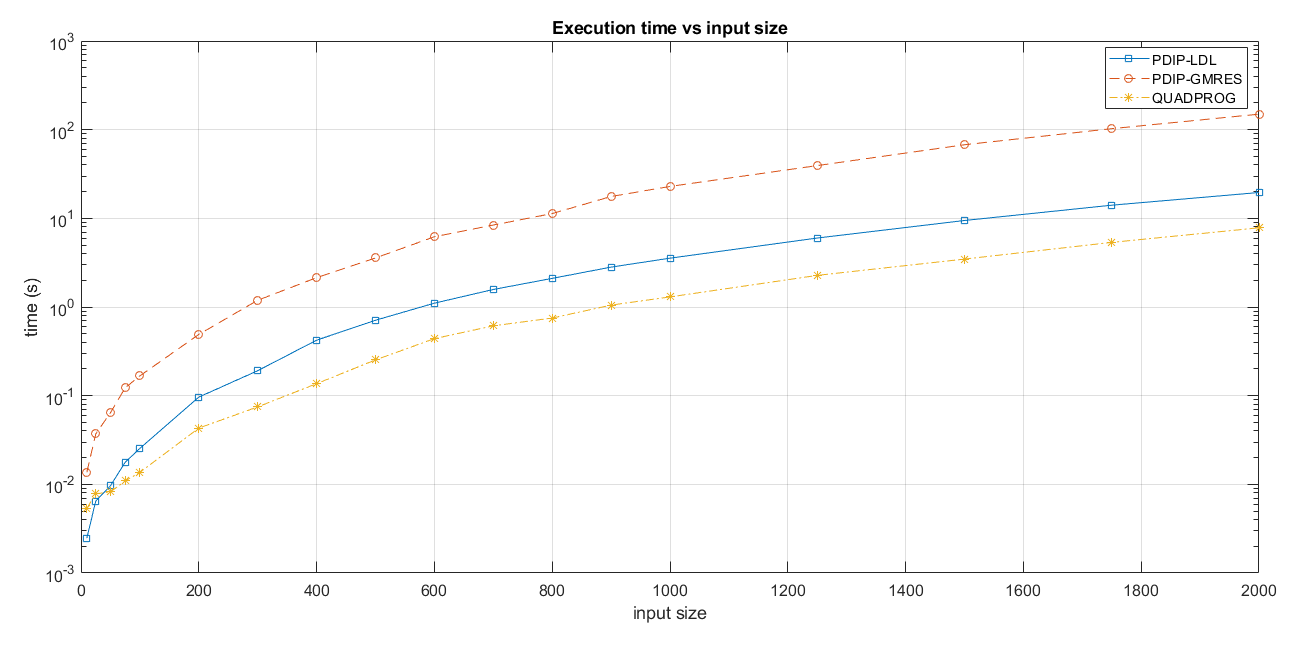
\includegraphics[height=4.52cm]{img/MU1.png}
    \caption{Confronto fra i tre metodi con asse delle y in \textit{log-scale}.\label{fig:exp111}}
    \end{subfigure}%
    ~ 
    \begin{subfigure}[h]{0.5\textwidth}
        \centering
                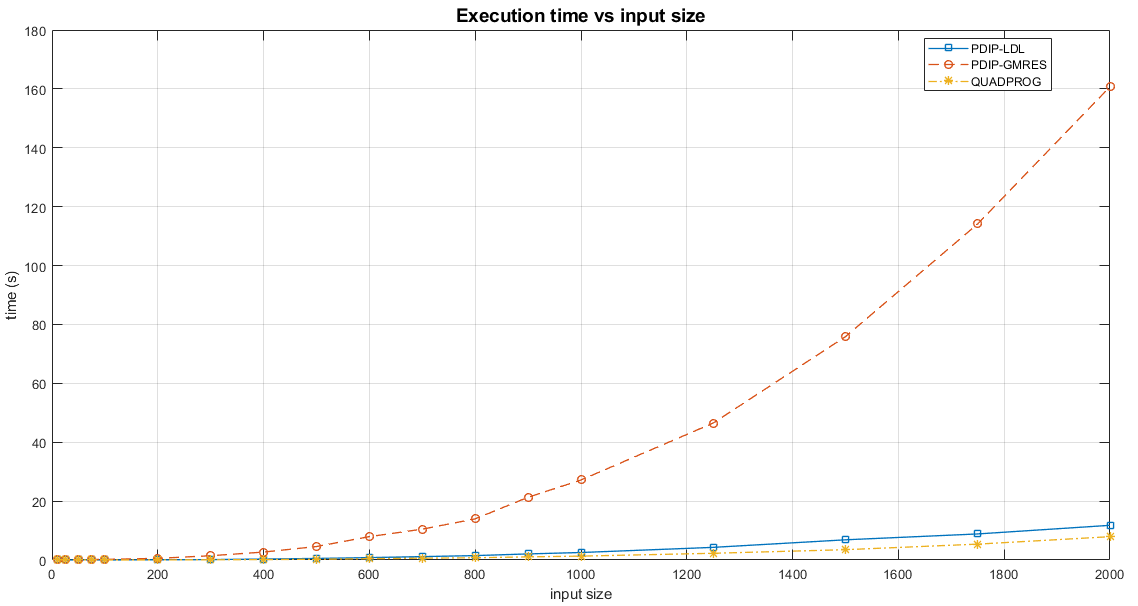
\includegraphics[height=4.4cm]{img/MU10.png}
    \caption{Confronto fra i tre metodi. \label{fig:exp112}}
    \end{subfigure}
    ~\newline
     \begin{subfigure}[h]{0.8\textwidth}
        \centering
                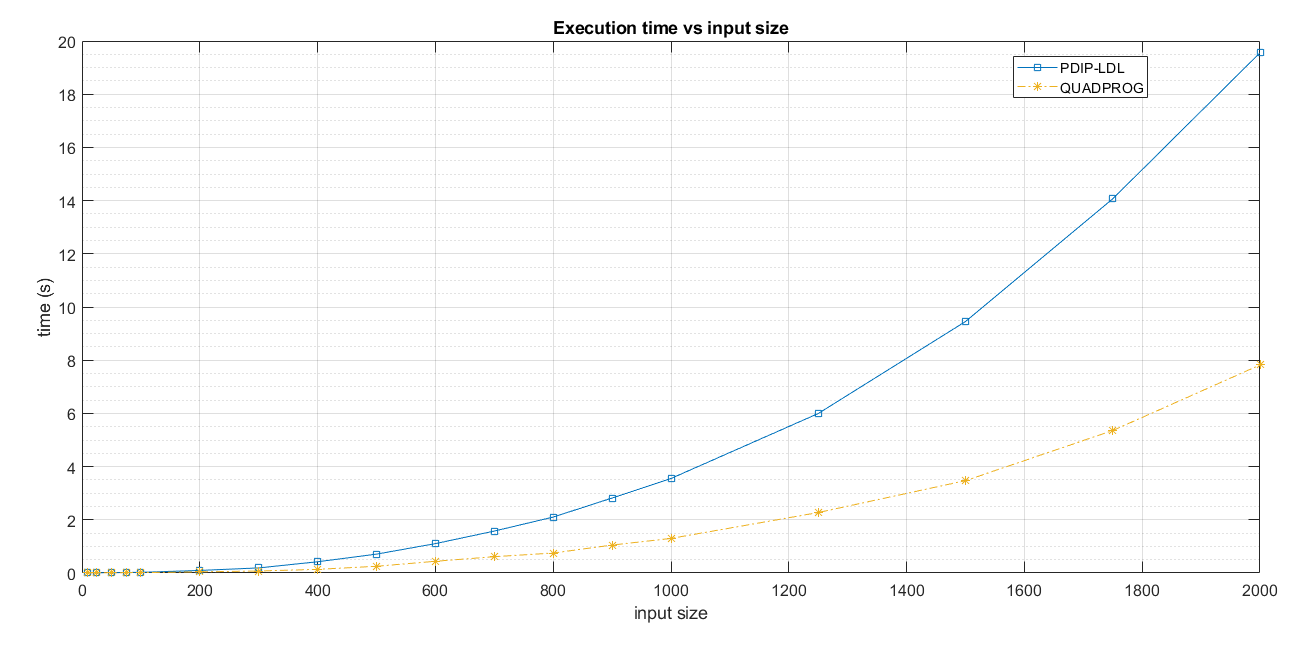
\includegraphics[height=6cm]{img/MU11.png}
    \caption{Grafico di confronto fra PIDP-LDL e QUADPROG. \label{fig:exp113}}
    \end{subfigure}
    \caption{I grafici mostra l'andamento del tempo di esecuzione, in secondi, all'aumentare della dimensione del problema $n$. \label{fig:exp1}}
\end{figure}


\begin{figure}[!h]
    \centering
    
\end{figure}

La Figura \ref{fig:exp1} ci permette di 

\begin{table}[!h]
\centering
\begin{tabular}{|l|c|c|c|c|c|c|c|c|}
\hline \textbf{input size}                  & \textbf{50}  & \textbf{75}  & \textbf{100} & \textbf{200}  & \textbf{300}  & \textbf{400}  & \textbf{500}  & \textbf{600}  \\\hline
\textbf{PDIP-LDL}                    & 0.0064       & 0.0177       & 0.0211       & 0.0575        & 0.1418        & 0.3251        & 0.5271        & 0.8170        \\
\textbf{QUADPROG}                    & 0.0069       & 0.0115       & 0.0137       & 0.0334        & 0.0737        & 0.1377        & 0.2590        & 0.4541        \\
\textbf{slowfactor} & \textbf{0.9259}       & 1.5432       & 1.5422       & 1.7229        & 1.9247        & \textbf{2.3617}        & 2.0351        & 1.7989        \\ \hline
\textbf{input size}                  & \textbf{700} & \textbf{800} & \textbf{900} & \textbf{1000} & \textbf{1250} & \textbf{1500} & \textbf{1750} & \textbf{2000} \\\hline
\textbf{PDIP-LDL}                    & 1.1532       & 1.4939       & 2.0655       & 2.5441        & 4.2911        & 6.8573        & 8.8513        & 11.7768       \\
\textbf{QUADPROG}                    & 0.6157       & 0.7584       & 1.0631       & 1.3172        & 2.2816        & 3.5041        & 5.3935        & 7.9170        \\
\textbf{\textit{slowfactor}} & 1.8728       & 1.9697       & 1.9428       & 1.9315        & 1.8808        & 1.9569        & 1.6411        & 1.4875  \\\hline     
\end{tabular}
    \caption{Tabelle contenenti la media dei tempi di esecuzione (s) di PDIP-LDL e QUADPROG relativi al primo sotto-esperimento. \label{tab:ldlqp2}}
    \end{table}
   
da anlizzare tempi di completamento:
\begin{itemize}
    \item GMRES più lento perchè metodo iterativo, andamento esponenziale
    \item LDL e QP prestazioni simili, slowfactor $\approx 2$
\end{itemize}
    
\begin{table}[!h]
\centering
\begin{tabular}{|l|c|c|c|c|c|c|c|c|}\hline
\textbf{input size} & \textbf{50}  & \textbf{75}  & \textbf{100} & \textbf{200}  & \textbf{300}  & \textbf{400}  & \textbf{500}  & \textbf{600}  \\\hline
\textbf{PDIP-LDL}   & 10.65\%      & 29.22\%      & 17.34\%      & 5.81\%        & 8.03\%        & 3.87\%        & 5.03\%        & 1.80\%        \\
\textbf{QUADPROG}   & 13.35\%      & 25.80\%      & 17.72\%      & 2.55\%        & 3.12\%        & 4.95\%        & 19.12\%       & 7.99\%        \\\hline
\textbf{input size} & \textbf{700} & \textbf{800} & \textbf{900} & \textbf{1000} & \textbf{1250} & \textbf{1500} & \textbf{1750} & \textbf{2000} \\\hline
\textbf{PDIP-LDL}   & 3.96\%       & 2.74\%       & 1.67\%       & 1.94\%        & 2.27\%        & 1.56\%        & 2.31\%        & 2.41\%        \\
\textbf{QUADPROG}   & 2.94\%       & 1.37\%       & 1.42\%       & 0.94\%        & 1.13\%        & 0.85\%        & 0.92\%        & 0.83\%     \\  \hline
\end{tabular}
    \caption{Tabella contenente la deviazione standard dei tempi di esecuzione di PDIP-LDL e QUADPROG relativi al primo sotto-esperimento. \label{tab:ldlqp1.1}}
\end{table}

descrizione grafico iterazioni in Fig. \ref{fig:exp1.2} aumenta sublinearmente nel nostro, costante in QP.

\begin{figure}[!h]
    \centering
    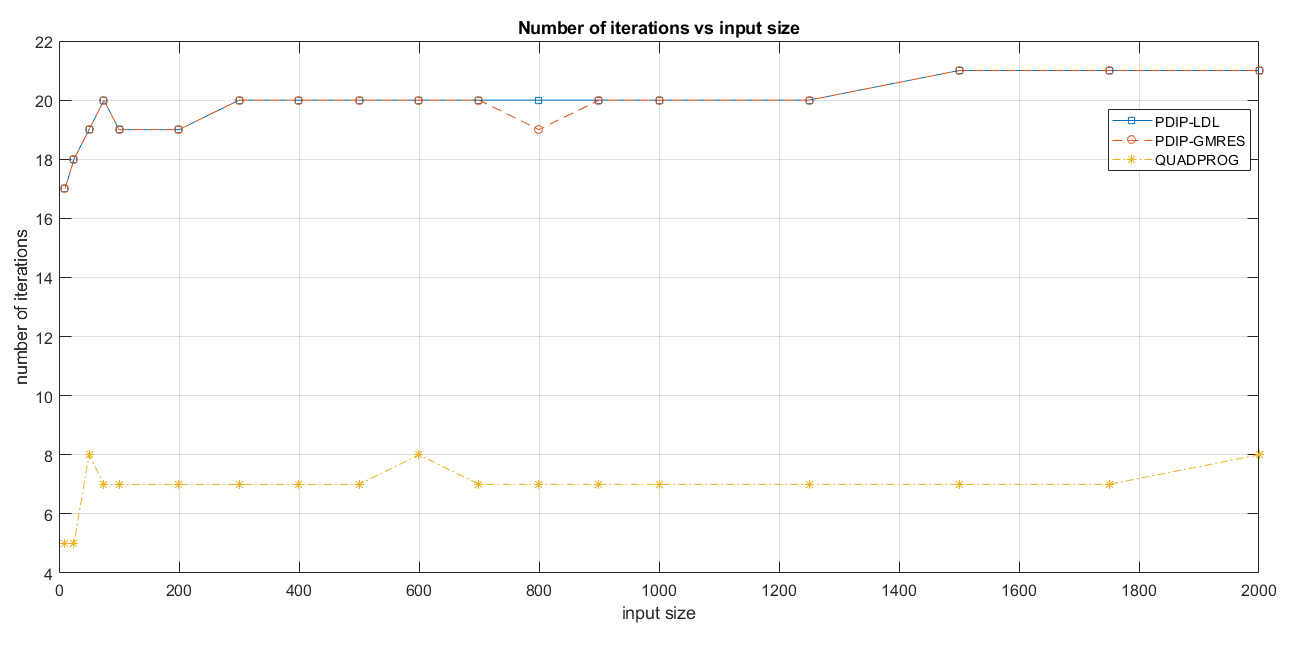
\includegraphics[width=\textwidth]{img/MU7.png}
    \caption{Il grafico mostra l'andamento del numero di iterazioni all'aumentare di $n$. \label{fig:exp1.2}}
\end{figure}

\subsection*{Numero di Vincoli}

 In questo gruppo di esperimenti abbiamo voluto analizzare l'effetto del numero di vincoli $m$ sul tempo di convergenza dei metodi; $\delta$ ed $n$ rimangono fissati come in Tab. \ref{tab:param}.

\begin{figure}[!h]
    \centering
    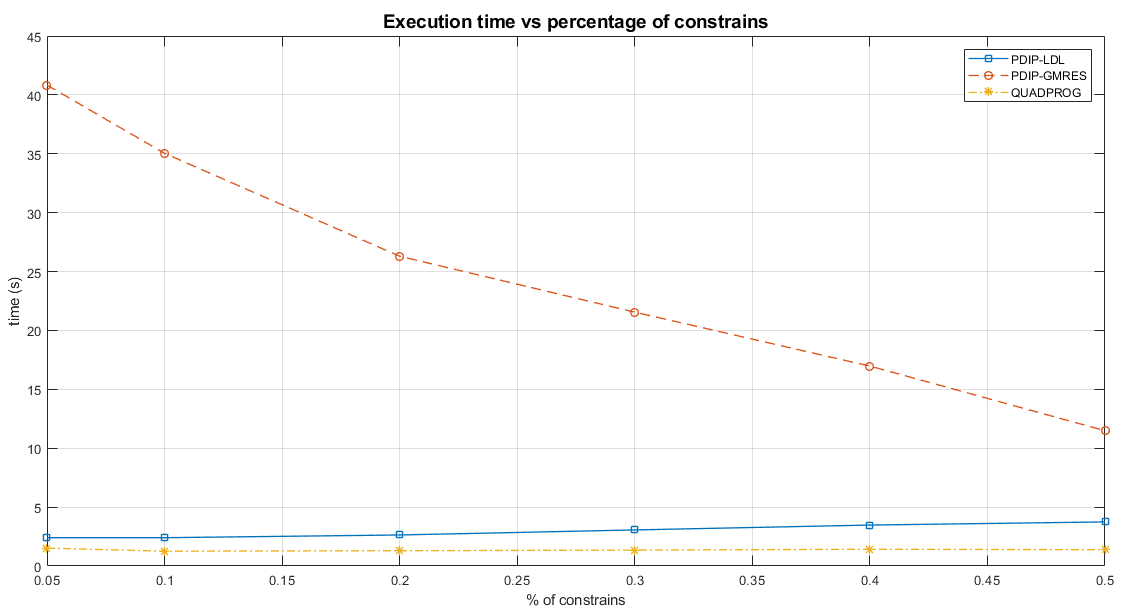
\includegraphics[width=\textwidth, height=7.5cm]{img/MU2.png}
    \caption{Il grafico mostra l'andamento del tempo di esecuzione all'aumentare del numero dei vincoli in $A$. \label{fig:exp2}}
\end{figure}
 
in generale in Fig. \ref{fig:exp2.1} GMRES sembra migliorare all'aumentare del numero di vincoli, forse perchè lavora meglio su sistemi lineari più grandi. Confrontando LDL e QP in Fig. \ref{fig:exp2.2} invece il nostro metodo accusa l'aumento del numero di vincoli mentre QP rimane più stabile, seppur comunque aumentando leggermente. 
 
\begin{figure}[!h]
    \centering
    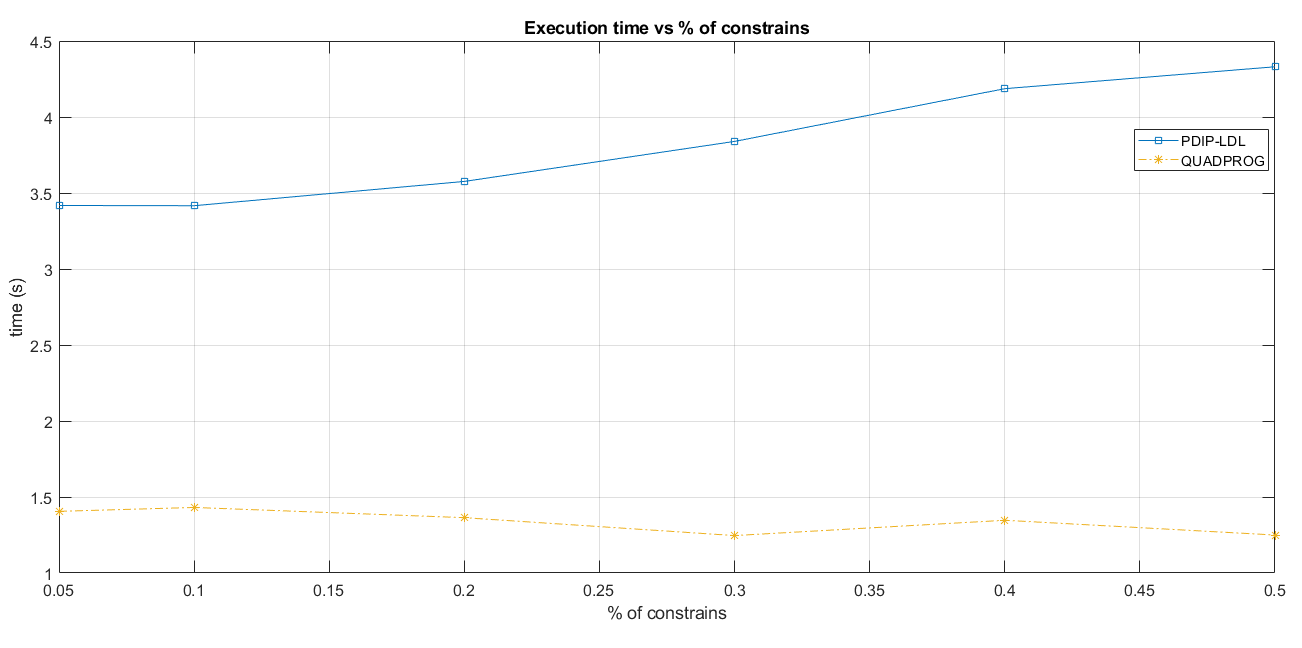
\includegraphics[width=\textwidth, height=7cm]{img/MU3.png}
    \caption{Grafico di confronto fra PIDP-LDL e QUDPROG. \label{fig:exp2.1}}
\end{figure}

slowfactor al massimo $2.5$

\begin{table}[!h]
\centering
\begin{tabular}{l|c|c|c|c|c|c}

$\mathbf{k/n}$            & \textbf{0.05} & \textbf{0.1} & \textbf{0.2} & \textbf{0.3} & \textbf{0.4} & \textbf{0.5} \\ \hline
\textbf{PDIP-LDL}                    & $2.401 \pm 2.6\%$       & $2.403 \pm 1.8\%$       & $2.634     \pm 2\%$   & $3.062 \pm 3\%$      & $3.476 \pm 1.9\%$      & $3.743 \pm 2.8\%$       \\
\textbf{QUADPROG}                    & $1.519 \pm 3.3\%$       & $1.256 \pm 2.4\%$       & $1.299 \pm 0.9\%$       & $1.351 \pm 1.6\%$       & $1.420 \pm 0.9\%$       & $1.382 \pm 3.6\%$       \\
\textbf{\textit{slowfactor}} &\textbf{1.581}        & 1.913       & 2.027       & 2.267       & 2.446       & \textbf{2.707} 
\end{tabular}
\caption{Tabella contenente media e deviazione standard dei tempi di esecuzione (s) di PDIP-LDL e QUADPROG relativi al secondo sotto-esperimento.\label{tab:ldlqp2}}
\end{table}

In Fig. \ref{fig:exp2.2} il numero iterazioni diminuisce all'aumentare di $m$, QP rimane sempre costante.


\begin{figure}[!h]
    \centering
    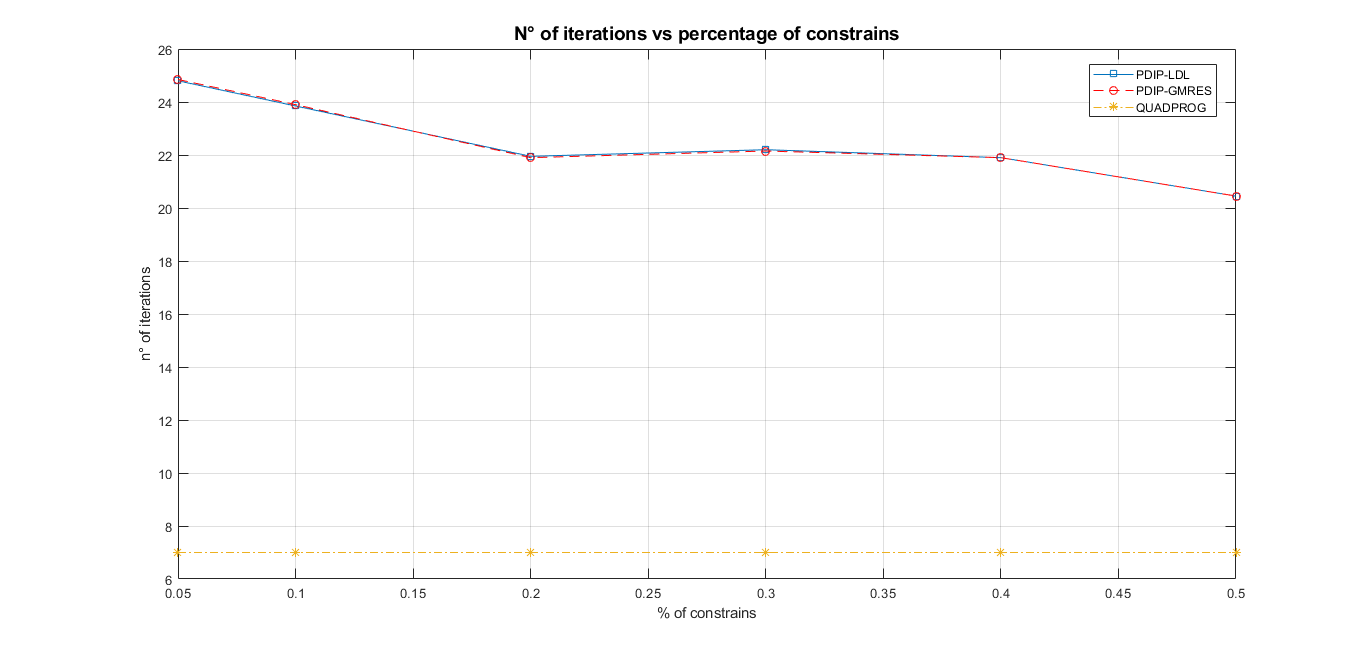
\includegraphics[width=\textwidth]{img/MU8.png}
    \caption{Il grafico mostra l'andamento del numero di iterazioni all'aumentare di $m$. \label{fig:exp2.2}}
\end{figure}


\subsection*{Densità}

 In questo gruppo di esperimenti abbiamo voluto testare qualora la densità della matrice $Q$ avesse effetti sui tempi di convergenza dei vari approcci coinvolti nella nostra analisi.

\begin{figure}[h]
    \centering
    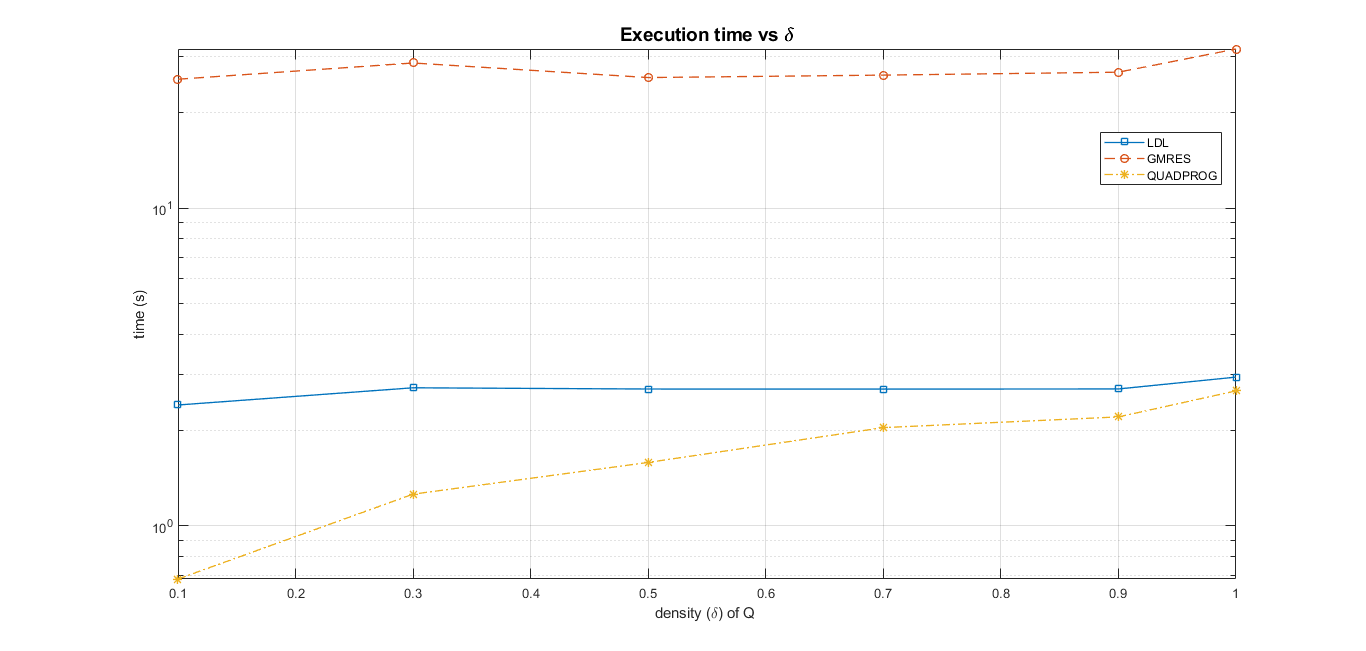
\includegraphics[width=\textwidth]{img/MU4.png}
    \caption{Il grafico mostra l'andamento del tempo di esecuzione (in \textit{log-scale} sull'asse delle y) all'aumentare della densità ($\delta$) di $Q$. \label{fig:exp3.1}}
\end{figure}
 
 Qui le nostre due implementazioni non sembrano risentire troppo dell'aumento di densità della matrice, con LDL migliore, mentre questo vale per QP dove il tempo di completamente aumenta. Iterazioni tutti costanti.


\begin{table}[!h]
\centering
\begin{tabular}{l|c|c|c|c|c|c}
\textbf{density}                     & \textbf{0.1} & \textbf{0.3} & \textbf{0.5} & \textbf{0.7} & \textbf{0.9} & \textbf{1.0} \\ \hline
\textbf{PDIP-LDL}                    & $2.401 \pm 1.2\%$       & $2.719 \pm 2.8\%$       & $2.695  \pm 2\%$       & $2.694 \pm 2.2\%$       & $2.696 \pm 2.3\%$       & $2.938  \pm 2.4\%$       \\
\textbf{QUADPROG}                    & $0.681  \pm 2.2\%$      & $1.258  \pm 5\%$       & $1.583 \pm 2.8\%$       & $2.038 \pm 1.5\%$       & $2.202 \pm 1.1\%$       & $2.659 \pm 5.9\%$       \\
\textbf{\textit{slowfactor}} & \textbf{3.526}       & 2.161       & 1.701       & 1.321       & 1.224       & \textbf{1.104}
\end{tabular}
\caption{Tabella contenente media e deviazione standard dei tempi di esecuzione (s) di PDIP-LDL e QUADPROG relativi al terzo sotto-esperimento. \label{tab:ldlqp3}}
\end{table}


\begin{figure}[!h]
    \centering
    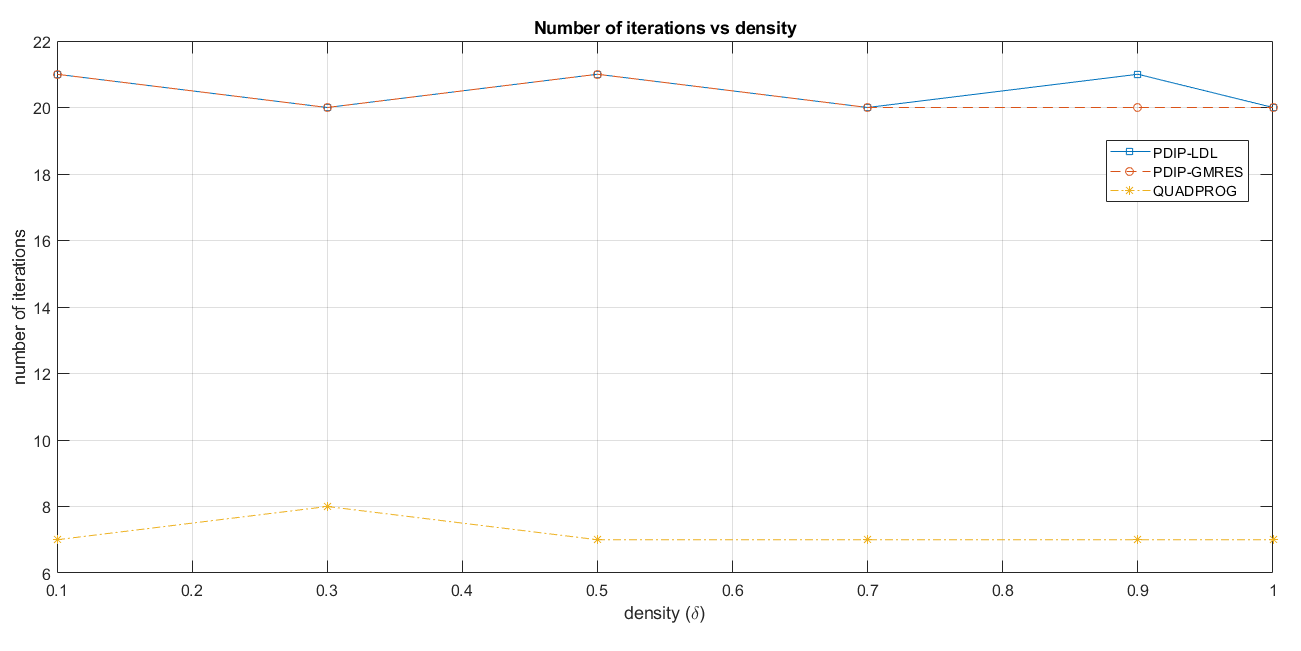
\includegraphics[width=\textwidth]{img/MU9.png}
    \caption{Il grafico mostra l'andamento del numero di iterazioni all'aumentare di $\delta$. \label{fig:exp3.2}}
\end{figure}

\subsection*{Convergenza e Accuratezza della Soluzione}


Gap collezionato solo per la nostra implementazione, decresce di un ordine di grandezza ad ogni iterazione.
\begin{figure}[h]
    \centering
    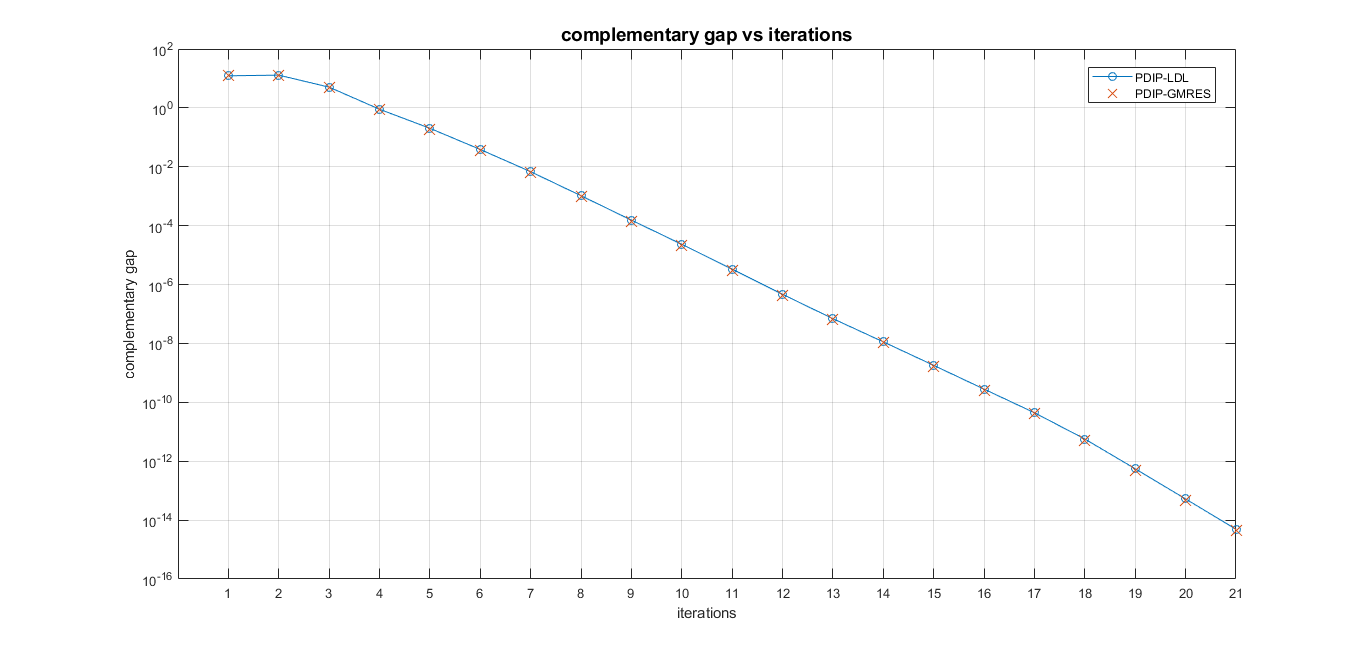
\includegraphics[width=\textwidth]{img/MU6.png}
    \caption{Il grafico mostra l'andamento del gap (in \textit{log-scale} sullasse delle y) all'aumentare delle iterazioni. \label{fig:gap}}
\end{figure}

e magari o una tabella o un grafico con
$$ \norm{x_{LDL} - x_{QUADPROG}} $$
$$ \norm{\nabla L_{LDL} - \nabla L_{QUADPROG}} $$
$$ \norm{\lambda_{LDL} - \lambda_{QUADPROG}} $$

\begin{table}[h!]
\centering
\begin{tabular}{c|c|l|c}
$\mathbf{\norm{\delta x}}$ & \multicolumn{2}{c|}{\textbf{PDIP-GMRES}}         & \textbf{QUADPROG}          \\ \hline
\textbf{PDIP-LDL}            & \multicolumn{2}{c|}{$3.3856\cdot10^{-13}\pm6\%$} & $4.3127\cdot10^{-3}\pm0\%$ \\ \hline
\textbf{PDIP-GMRES}          & \multicolumn{2}{c|}{}                            & $4.3127\cdot10^{-3}\pm0\%$
\end{tabular}
\caption{Media e deviazione standard, sulle 20 ripetizioni, della norma della differenza fra i vettori soluzione $\deltax$\label{tab:normx}}
\end{table}

\begin{table}[!h]
\begin{tabular}{c|c|c|c|c|}
                   & \multicolumn{2}{c|}{\textbf{PDIP-LDL}}                                        & \multicolumn{2}{c|}{\textbf{PDIP-GMRES}}                                      \\ \hline
\textbf{PDIP-GMRES} & $1.6224\cdot10^{-13}\pm11\%$          & $1.1201\cdot10^{-12}\pm5.4\%$         & \multicolumn{2}{c|}{ }                                                        \\ 
\textbf{QUADPROG}   & $1.5712\cdot10^{-3}\pm0\%$            & $5.3517\cdot10^{-3}\pm0\%$            & $1.5712\cdot10^{-3}\pm0\%$            & $5.3517\cdot10^{{-3}}\pm0\%$          \\
                    & $\norm{ \delta\lambda_{eqlin} }$ & $\norm{ \delta\lambda_{s} }$ & $\norm{ \delta\lambda_{eqlin} }$ & $\norm{ \delta\lambda_{s} }$
\end{tabular}
\caption{Media e deviazione standard, sulle 20 ripetizioni, della norma della differenza fra i moltiplicatori lagrangiani risultanti $\delta\lambda$\label{tab:norml}}
\end{table}